\documentclass{report}

\usepackage{amssymb}
\usepackage{amsmath}
\usepackage{amsthm}
\usepackage{kpfonts}
\usepackage{tikz}
\usepackage{wrapfig}
\usepackage{amsmath}
\usepackage{epigraph}
\usepackage{lipsum}

\renewcommand\epigraphflush{flushright}
\renewcommand\epigraphsize{\normalsize}
\setlength\epigraphwidth{0.7\textwidth}

\definecolor{titlepagecolor}{cmyk}{1,.60,0,.40}

\DeclareFixedFont{\titlefont}{T1}{ppl}{b}{it}{0.5in}

\makeatletter                       
\def\printauthor{%                  
    {\large \@author}}              
\makeatother

% The following code is borrowed from: http://tex.stackexchange.com/a/86310/10898

\newcommand\titlepagedecoration{%
\begin{tikzpicture}[remember picture,overlay,shorten >= -10pt]

\coordinate (aux1) at ([yshift=-15pt]current page.north east);
\coordinate (aux2) at ([yshift=-410pt]current page.north east);
\coordinate (aux3) at ([xshift=-4.5cm]current page.north east);
\coordinate (aux4) at ([yshift=-150pt]current page.north east);

\begin{scope}[titlepagecolor!40,line width=12pt,rounded corners=12pt]
\draw
  (aux1) -- coordinate (a)
  ++(225:5) --
  ++(-45:5.1) coordinate (b);
\draw[shorten <= -10pt]
  (aux3) --
  (a) --
  (aux1);
\draw[opacity=0.6,titlepagecolor,shorten <= -10pt]
  (b) --
  ++(225:2.2) --
  ++(-45:2.2);
\end{scope}
\draw[titlepagecolor,line width=8pt,rounded corners=8pt,shorten <= -10pt]
  (aux4) --
  ++(225:0.8) --
  ++(-45:0.8);
\begin{scope}[titlepagecolor!70,line width=6pt,rounded corners=8pt]
\draw[shorten <= -10pt]
  (aux2) --
  ++(225:3) coordinate[pos=0.45] (c) --
  ++(-45:3.1);
\draw
  (aux2) --
  (c) --
  ++(135:2.5) --
  ++(45:2.5) --
  ++(-45:2.5) coordinate[pos=0.3] (d);   
\draw 
  (d) -- +(45:1);
\end{scope}
\end{tikzpicture}%
}

\usetikzlibrary{shapes.geometric, arrows}

\tikzstyle{block} = [rectangle, draw, fill=blue!20, 
    text width=7em, text centered, rounded corners, minimum height=4em]
\tikzstyle{line} = [draw, -latex']

\DeclareMathOperator{\lcm}{lcm}
\DeclareMathOperator{\im}{im}

\title{Group Theory}
\author{Jacob Denson}
\date{\today}

\begin{document}
\begin{titlepage}
\noindent
\titlefont Artificial Intelligence:\\Reinforcement\\Learning\par
\epigraph{How do we design machines that are able to act at the same capability of a human being. This report attempts to address this question. Knowledge of elementary probability theory will be assumed.}
\null\vfill
\vspace*{1cm}
\noindent
\hfill
\begin{minipage}{0.35\linewidth}
    \begin{flushright}
        \printauthor
    \end{flushright}
\end{minipage}
%
\begin{minipage}{0.02\linewidth}
    \rule{1pt}{125pt}
\end{minipage}
\titlepagedecoration
\end{titlepage}

\chapter{What is AI?}

Artificial Intelligence is the science of designing intelligent agents -- actors on an environment. How do we define intelligence? In this class we define it to be the capability to achieve goals in the world. We do not spend time philosophically adressing this question. This definition thus becomes a tool rather than a philosophy -- we can actually measure our intelligence.

By using this definition, it becomes simple to test whether a machine is intelligent. Given a task, we define a performance metric. An intelligent machine is one that scores relatively high on this metric. Rationality is choosing the optimal decisions given what it knows in order to maximize the metric. An important biproduct of the definition is that we do not need to understand how an agent works in order to understand why it is intelligent: Any strategy is fair game. If you would rather understand how the computation of a human brain works, artificial intelligence is not the field for you - take up computational neuroscience instead.

To be more specific, we define an agent as anything which can percieve an environment and act accordingly. An agent acts through its actuators, and percieves with its perceptions extracted from the environment, as shown in the diagram below. A percept sequence is the sequence of perceptions that an agent percieves. This should be (and has to be) all that an agent needs to make a rational decision. An agent function maps a percept sequence to an action -- it corresponds to the agent making a decision. The way an agent behaves induces a sequence of actions which we can evaluate with a performance metric. The metric should be designed such that a rational agent, which selects the action expected to maximize its performance metric given the percept sequence and all built-in knowledge the agent has, should behave completely correctly in its environment. Note that a rational agent is not omniscient -- it does not need to act in the best way given full knowledge of the environment, but the best expected knowledge given previous knowledge.

\begin{center}
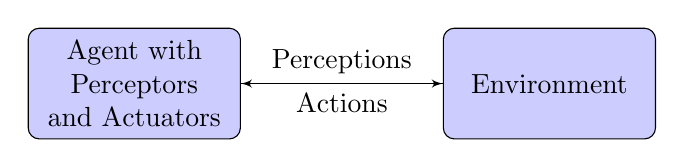
\begin{tikzpicture}[node distance = 10cm, auto]
    % Place nodes
    \node [block] (environment) {Environment};
    \node [block, left of=environment, node distance=15em] (agent) {Agent with Perceptors\\and Actuators};
    % Draw edges
    \path [line] (agent) -- node {Perceptions} (environment);
    \path [line] (environment) -- node {Actions} (agent);
\end{tikzpicture}
\end{center}

People may object to the definition established -- a pocket calculator shouldn't be intelligent just because it responds intelligently to an input. We respond by stating that intelligence is relative, a pocket calculator is more intelligent that an abacus. Human intelligence is just the ability to be capable on the range of tasks a human is able to do well in.

One case study to aid in this understanding is Turing's definition of artificial intelligence via his `Turing test'. A human interrogator attempts to determine whether the machine he is talking into has a human on the other side, or a robot impersonator. A machine is more intelligent than another if it tricks more people on average into thinking that it is a human. We do not care how the machine does it, as all aspects of the machine are hidden to the interrogator, but we do want the task to be performed as best as possible.

There are many aspects to building intellligence. We list the main topics here:

\begin{itemize}
  \item Decision Making
  \item Learning
  \item Planning
  \item Representation of Knowledge
\end{itemize}

Early on, planning and representation were important, whereas recently decisions and learning have gained more importance. Though we will touch on the first two, we will mainly focus on decisions and learning, using the others to supplement the learning process.

\section{Environments}

Environments come in various shapes and sizes. We list various qualities here:

\begin{itemize}
  \item A fully observable environment is an environment where all knowledge required and relevant to the agent is seen by its perceptors -- that is, its whole state is known. A partially observable environment is where some relevant information is know, and a unobservable environment is where an agent has no sensors to detect the environment.
  \item A single agent environment contains one agent interacting with the environment. A multiagent environment contains numerous agents all interacting to achieve their goal. Agents should be considered actors that modify their actions to maximize a performance metric. Not all agents may be following the same performance metric. In a multiagent environment, agents may be competitive, where an agents performance metric is maximized by minimizing all other agents metrics. Cooperative environments involve actions that maximize the performance metric of all other agents involve.
  \item In deterministic environments, an agents actions result in direct results in the environment. Stochastic or nondeterministic environments give uncertain results to an agents actions. This may be do to the random nature of the task or the unobtainable knowledge of the task.
  \item Episodic environments are environments where an agents percept sequence may be divided into atomic episodes where decisions in one episode do not impact the other. Continuous environments cannot be.
  \item An environment is static if it does not change when an agent is deciding actions to take. A dynamic environment can be seen as continually asking the agent to perform at all available times, and acting as if the agent chose to do nothing if it does not respond instantaneously.
  \item Discrete environments work in a finite or countable way. Continuous environments have the quality of a stream of states, action, or time associated with them.
\end{itemize}

The main focus in this class will be stochastic, single agent, discrete environments. Episodic and continuous tasks will both be considered.

\chapter{Utility?}

Though the metric assigned to an agent's performance may not be given, the agent may still have a way to approximate this metric in order to perform better. A football team choose to play defensively when they know their metric is higher than the other teams. We call this a utility. 
Though we know the current metric in some problems in football match, this is not the fully calculate metric so is a utility. It would be almost unobtainable to get a full metric before decisions are made in all but the simplest environments.

One method an agent may attempt to obtain rationality is to rank various agent functions by a preference such that the top preference corresponds to an optimal score with the metric. Utility theory attempts to represent and reason with preferences. Decision theory takes uncertainty into account. The main problem is to choose the action that yields the hgihest expected utility, averaged over all outcomes of an outcome. Control theory takes a dynamic approach to maximizing the utility function over time. We will use many the ideas from these fields to organize the theory of reinforcement learning.

\end{document}